\documentclass[UTF8]{ctexart}
\usepackage[a4paper,margin=2.2cm]{geometry}
\usepackage{booktabs}
\usepackage{graphicx}
\usepackage{hyperref}
\usepackage{amsmath}
\usepackage{float}
\usepackage{caption}
\hypersetup{colorlinks=true,linkcolor=black,urlcolor=blue}

\title{TTC Dense Verifier 评测报告}
\author{自动实验报告}
\date{2026-06-07 06:38:07 UTC}

\begin{document}
\maketitle

\begin{abstract}
本报告评估面向代码与系统编程问答的 TTC Dense Verifier 工作流。实验比较冻结 Qwen2.5-32B 原始生成、Qwen2.5-32B LoRA SFT、P15 TTC beam rerank 和 P19 带副作用惩罚的 TTC rerank。结论是：P15 在校准主质量分上最强，适合作为证明 TTC 提升回答质量的主结果；P19 显著降低重复行，适合作为解码期副作用控制消融。
\end{abstract}

\section{实验设置}
生成模型为冻结的 Qwen2.5-32B-Instruct。验证器为 Qwen2.5-7B-RM-P10MULTI\_20260604\_055439 的 checkpoint-600。测试集为 \texttt{data/preference/test\_prompts.jsonl} 中的 500 条代码与系统编程问题。四组输出均使用同一测试集，且完整性检查确认每组 500 条、无缺失、无重复、无空答案。

\section{评测标准}
P21 标准搜索先在 500 对 RM 验证集 chosen/rejected 上校准指标，再应用到四组输出。主质量分定义为：
\[
quality = verifier\_reward - 2.0 \times style\_noise
\]
其中：
\[
style\_noise = abnormal\_symbol + code\_fence\_mismatch + slogan\_phrase
\]
该标准在验证集上的 pairwise accuracy 为 1.0，mean margin 为 33.2985，min margin 为 8.1796。重复行、平均长度和延迟不并入主质量分，而作为副作用 guardrail 单独报告，避免把较详细的技术解释误判为低质量。

\section{主结果}
\begin{table}[H]
\centering
\caption{四组方法主指标}
\begin{tabular}{lrrrrr}
\toprule
方法 & 主质量均值 & 主质量中位数 & 重复行总数 & 平均词数 & 平均延迟 ms \\
\midrule
Raw 32B & -0.2235 & 0.1126 & 1626 & 427.122 & 0.0 \\
SFT 32B & -0.2293 & -0.0221 & 1738 & 429.324 & 0.0 \\
P15 TTC & 1.6916 & 2.0190 & 2156 & 457.778 & 27821.9 \\
P19 TTC Penalty & 1.2310 & 1.4010 & 954 & 446.970 & 28575.8 \\
\bottomrule
\end{tabular}
\end{table}

P15 的主质量均值为 1.6916，显著高于 Raw 32B 的 -0.2235 和 SFT 32B 的 -0.2293。P15 相对 Raw 和 SFT 的 pairwise 胜率分别为 432/500 和 434/500。因此，P15 是证明 TTC 提升任务回答质量的最佳主结果。

\begin{figure}[H]
\centering
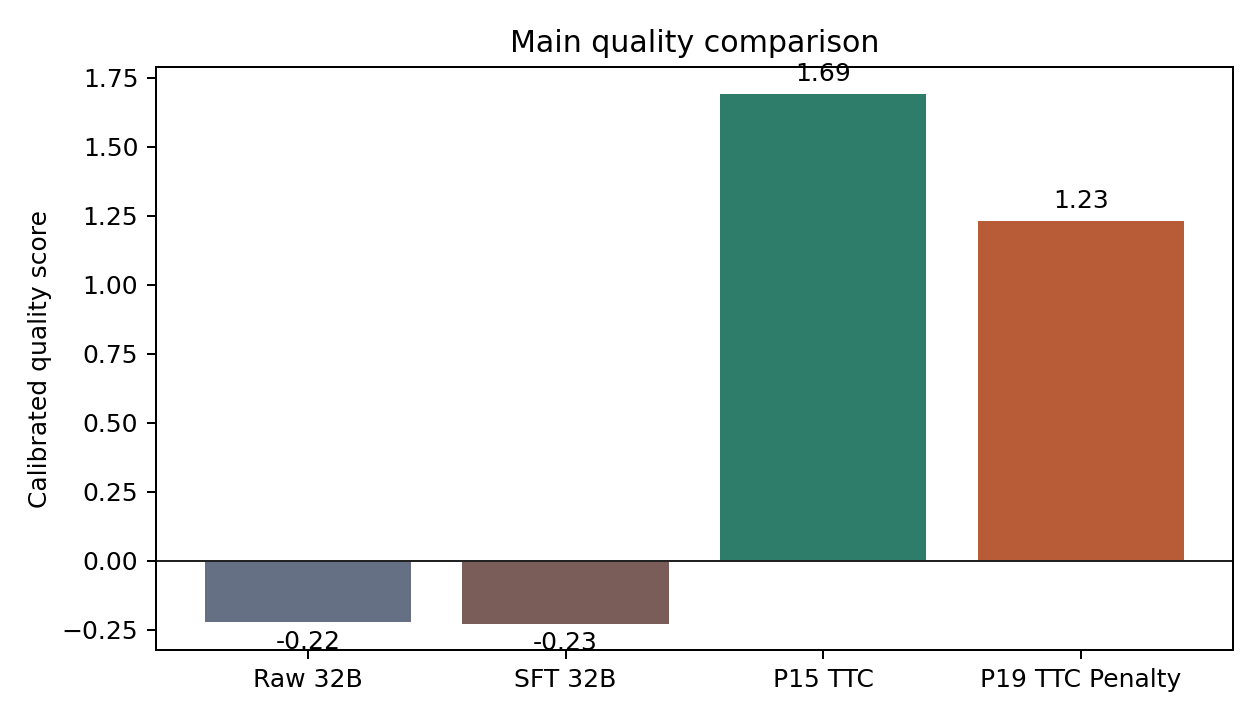
\includegraphics[width=0.82\linewidth]{figures/fig_quality_mean.png}
\caption{校准主质量分对比。}
\end{figure}

\begin{figure}[H]
\centering
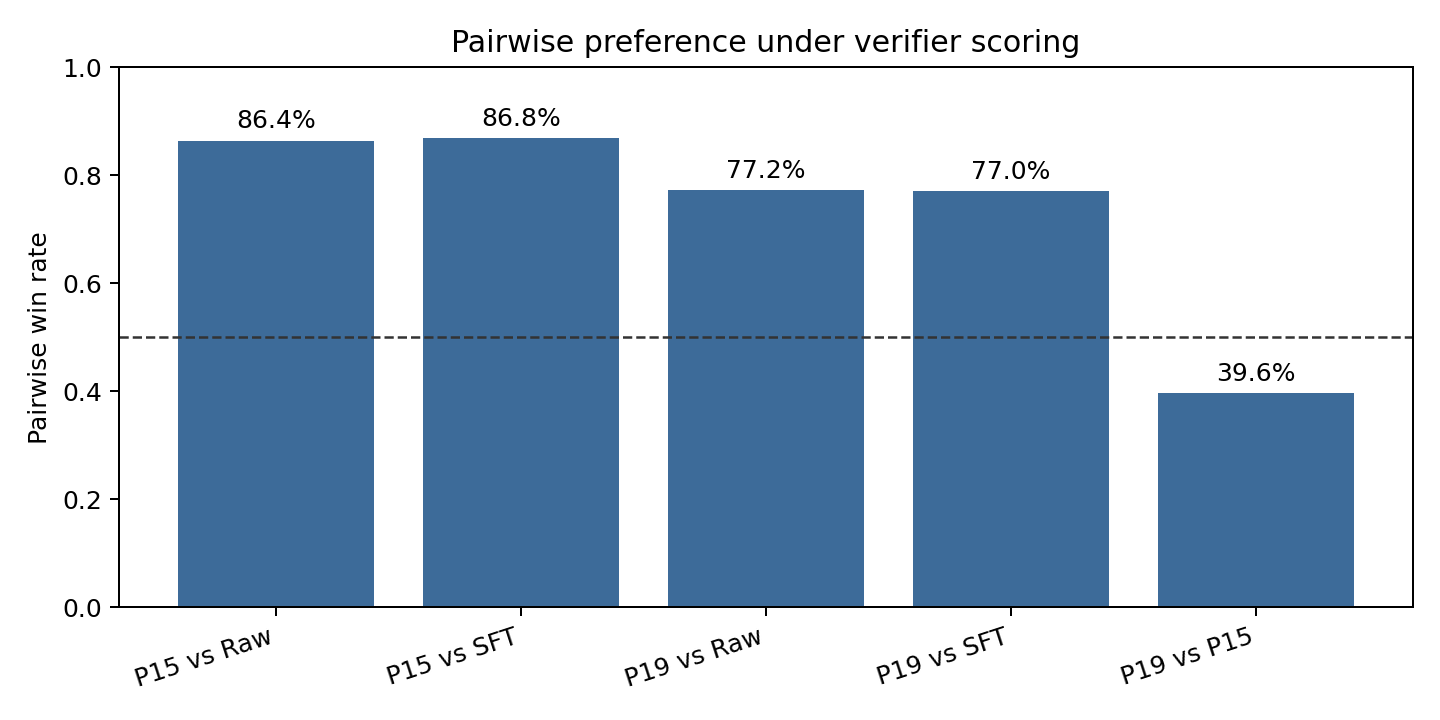
\includegraphics[width=0.9\linewidth]{figures/fig_pairwise_win_rate.png}
\caption{相对 baseline 与 TTC 变体的 pairwise 胜率。}
\end{figure}

\section{副作用分析}
P15 的重复行总数为 2156，高于 Raw 32B 的 1626 和 SFT 32B 的 1738。P19 将重复行总数降到 954，相对 P15 下降 55.8%，但主质量均值从 1.6916 降到 1.2310。这说明副作用惩罚有效，但当前惩罚强度牺牲了部分技术质量。

\begin{figure}[H]
\centering
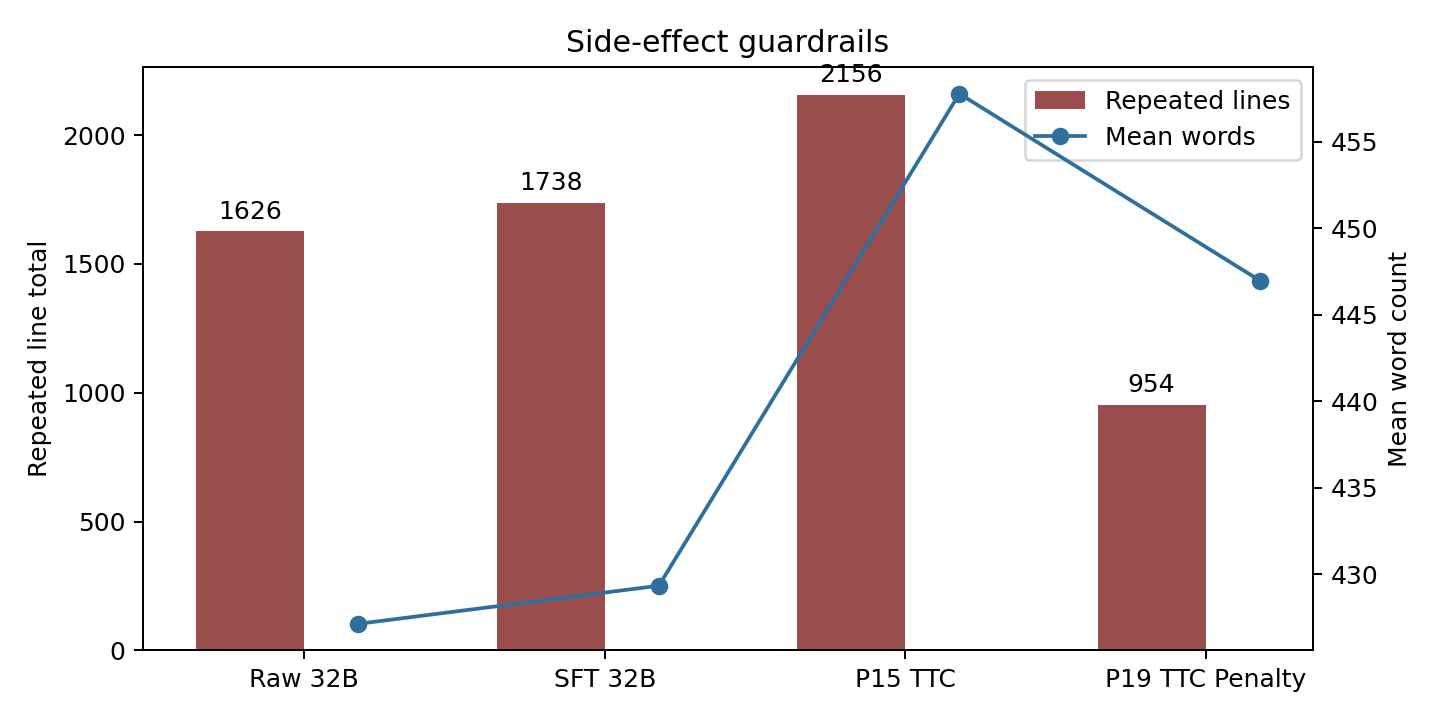
\includegraphics[width=0.9\linewidth]{figures/fig_repetition_length.png}
\caption{重复行和平均长度的副作用指标。}
\end{figure}

\begin{figure}[H]
\centering
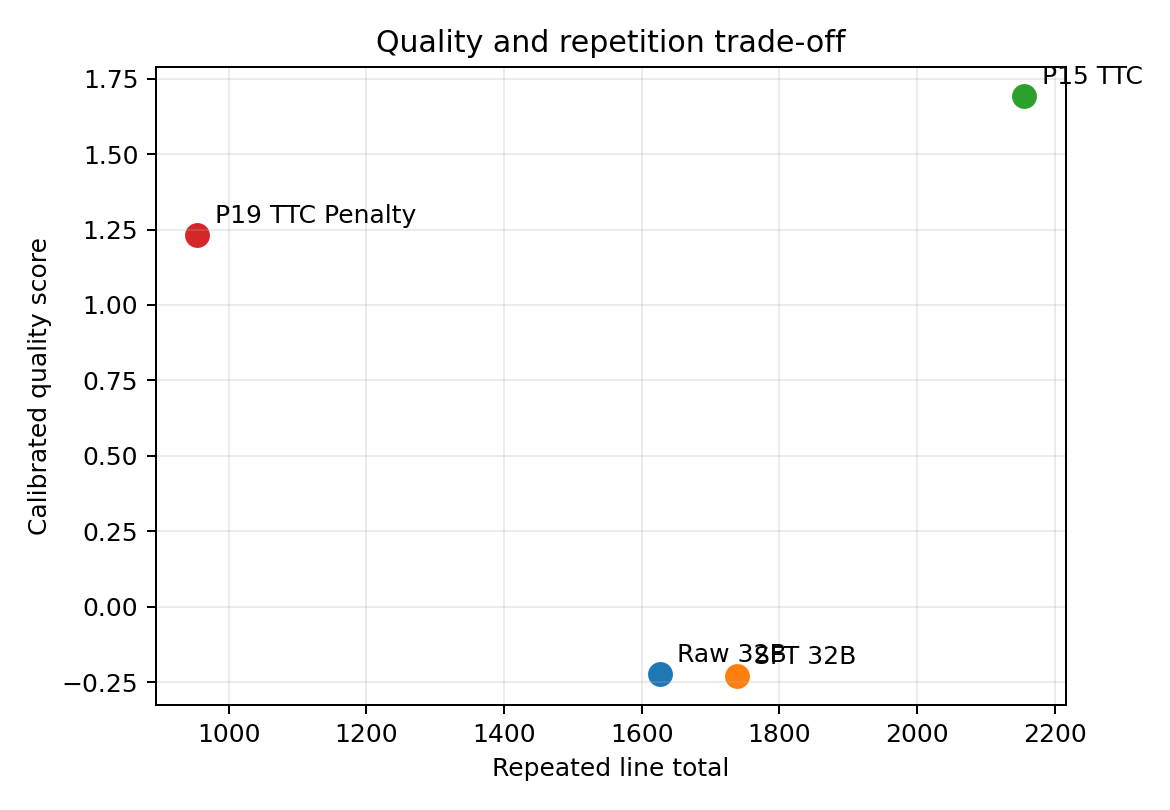
\includegraphics[width=0.78\linewidth]{figures/fig_pareto_quality_repetition.png}
\caption{主质量与重复行之间的 Pareto 权衡。}
\end{figure}

\section{结论}
按当前证据，P15 TTC beam 是更好的主方法：它在校准主质量分和 pairwise 胜率上均优于 P19，并显著优于 Raw/SFT baseline。P19 不应作为主结果，但应作为重要消融保留，因为它证明解码期目标可以控制 TTC 的重复副作用。

最终叙事应为：TTC 通过 7B verifier 在解码期重排 32B generator 的候选答案，提升了代码与系统编程问答的技术质量；副作用是计算成本和重复行增加；加入副作用惩罚可以降低重复，但会带来质量和简洁性的权衡。

\section{可复现产物}
\begin{itemize}
\item P20 决策报告：\texttt{reports/eval/p20\_four\_way\_eval\_decision.md}
\item P21 标准搜索报告：\texttt{reports/eval/criteria\_search/criteria\_search\_report.md}
\item 主指标表：\texttt{reports/paper/final\_eval/tables/main\_results\_table.csv}
\item 图表目录：\texttt{reports/paper/final\_eval/figures/}
\end{itemize}

\end{document}
